\newcounter{english}
\documentclass{article}

% packages
\usepackage{amsmath, amsthm, thmtools, amsfonts, amssymb, luacode, catchfile, tikzducks, hyperref, ifthen}
\ifcsname c@kobocompile\endcsname
	\usepackage[a5paper, total={1072pt, 1448pt}, margin=10pt, includeheadfoot]{geometry} % set page margins
\else
	\usepackage[a4paper, margin=50pt, includeheadfoot]{geometry}
\fi
\usepackage[shortlabels]{enumitem}
\usepackage[skip=3pt, indent=0pt]{parskip}

% language
\usepackage[bidi=basic, layout=tabular, provide=*]{babel}
\ifcsname c@english\endcsname
	\babelprovide[main, import]{english}
\else
	\babelprovide[main, import]{hebrew}
	\babelprovide{rl}
\fi
%\babelfont{rm}{Libertinus Serif}
\babelfont{rm}[Renderer=Harfbuzz]{Libertinus Serif}
\babelfont{sf}{Libertinus Sans}
\babelfont{tt}{Libertinus Mono}

% style
\AddToHook{cmd/section/before}{\clearpage}	% Add line break before section
\linespread{1.3}
\setcounter{secnumdepth}{0}		% Remove default number tags from sections, this won't do well with theorems
\AtBeginDocument{\setlength{\belowdisplayskip}{3pt}}
\AtBeginDocument{\setlength{\abovedisplayskip}{3pt}}
\graphicspath{ {../images/} }

% operators
\DeclareMathOperator\cis{cis}
\DeclareMathOperator\Sp{Sp}
\DeclareMathOperator\tr{tr}
\DeclareMathOperator\im{Im}
\DeclareMathOperator\re{Re}
\DeclareMathOperator\diag{diag}
\DeclareMathOperator*\lowlim{\underline{lim}}
\DeclareMathOperator*\uplim{\overline{lim}}
\DeclareMathOperator\rng{rng}
\DeclareMathOperator\Sym{Sym}
\DeclareMathOperator\Arg{Arg}
\DeclareMathOperator\Log{Log}
\DeclareMathOperator\dom{dom}
\DeclareMathOperator\supp{Supp}
\DeclareMathOperator\var{Var}
\DeclareMathOperator\cov{Cov}

% commands
%\renewcommand\qedsymbol{\textbf{מש''ל}}
%\renewcommand\qedsymbol{\fbox{\emoji{lizard}}}
\newcommand{\Aa}[0]{\mathcal{A}}
\newcommand{\Bb}[0]{\mathcal{B}}
\newcommand{\CC}[0]{\mathbb{C}}
\newcommand{\Cc}[0]{\mathcal{C}}
\newcommand{\EE}[0]{\mathbb{E}}
\newcommand{\FF}[0]{\mathbb{F}}
\newcommand{\Ff}[0]{\mathcal{F}}
\newcommand{\Ii}[0]{\mathcal{I}}
\newcommand{\Gg}[0]{\mathcal{G}}
\newcommand{\Ll}[0]{\mathcal{L}}
\newcommand{\Mm}[0]{\mathcal{M}}
\newcommand{\NN}[0]{\mathbb{N}}
\newcommand{\Nn}[0]{\mathcal{N}}
\newcommand{\PP}[0]{\mathbb{P}}
\newcommand{\Pp}[0]{\mathcal{P}}
\newcommand{\QQ}[0]{\mathbb{Q}}
\newcommand{\RR}[0]{\mathbb{R}}
\newcommand{\Rr}[0]{\mathcal{R}}
\newcommand{\Ss}[0]{\mathcal{S}}
\newcommand{\TT}[0]{\mathbb{T}}
\newcommand{\Uu}[0]{\mathcal{U}}
\newcommand{\Vv}[0]{\mathcal{V}}
\newcommand{\Ww}[0]{\mathcal{W}}
\newcommand{\ZZ}[0]{\mathbb{Z}}
\newcommand{\acts}[0]{\circlearrowright}
\newcommand{\explain}[2] {
	\begin{flalign*}
		 && \text{#2} && \text{#1}
	\end{flalign*}
}
\newcommand{\maketitleprint}[0]{ \begin{center}
	%\begin{tikzpicture}[scale=3]
	%	\duck[graduate=gray!20!black, tassel=red!70!black]
	%\end{tikzpicture}	
	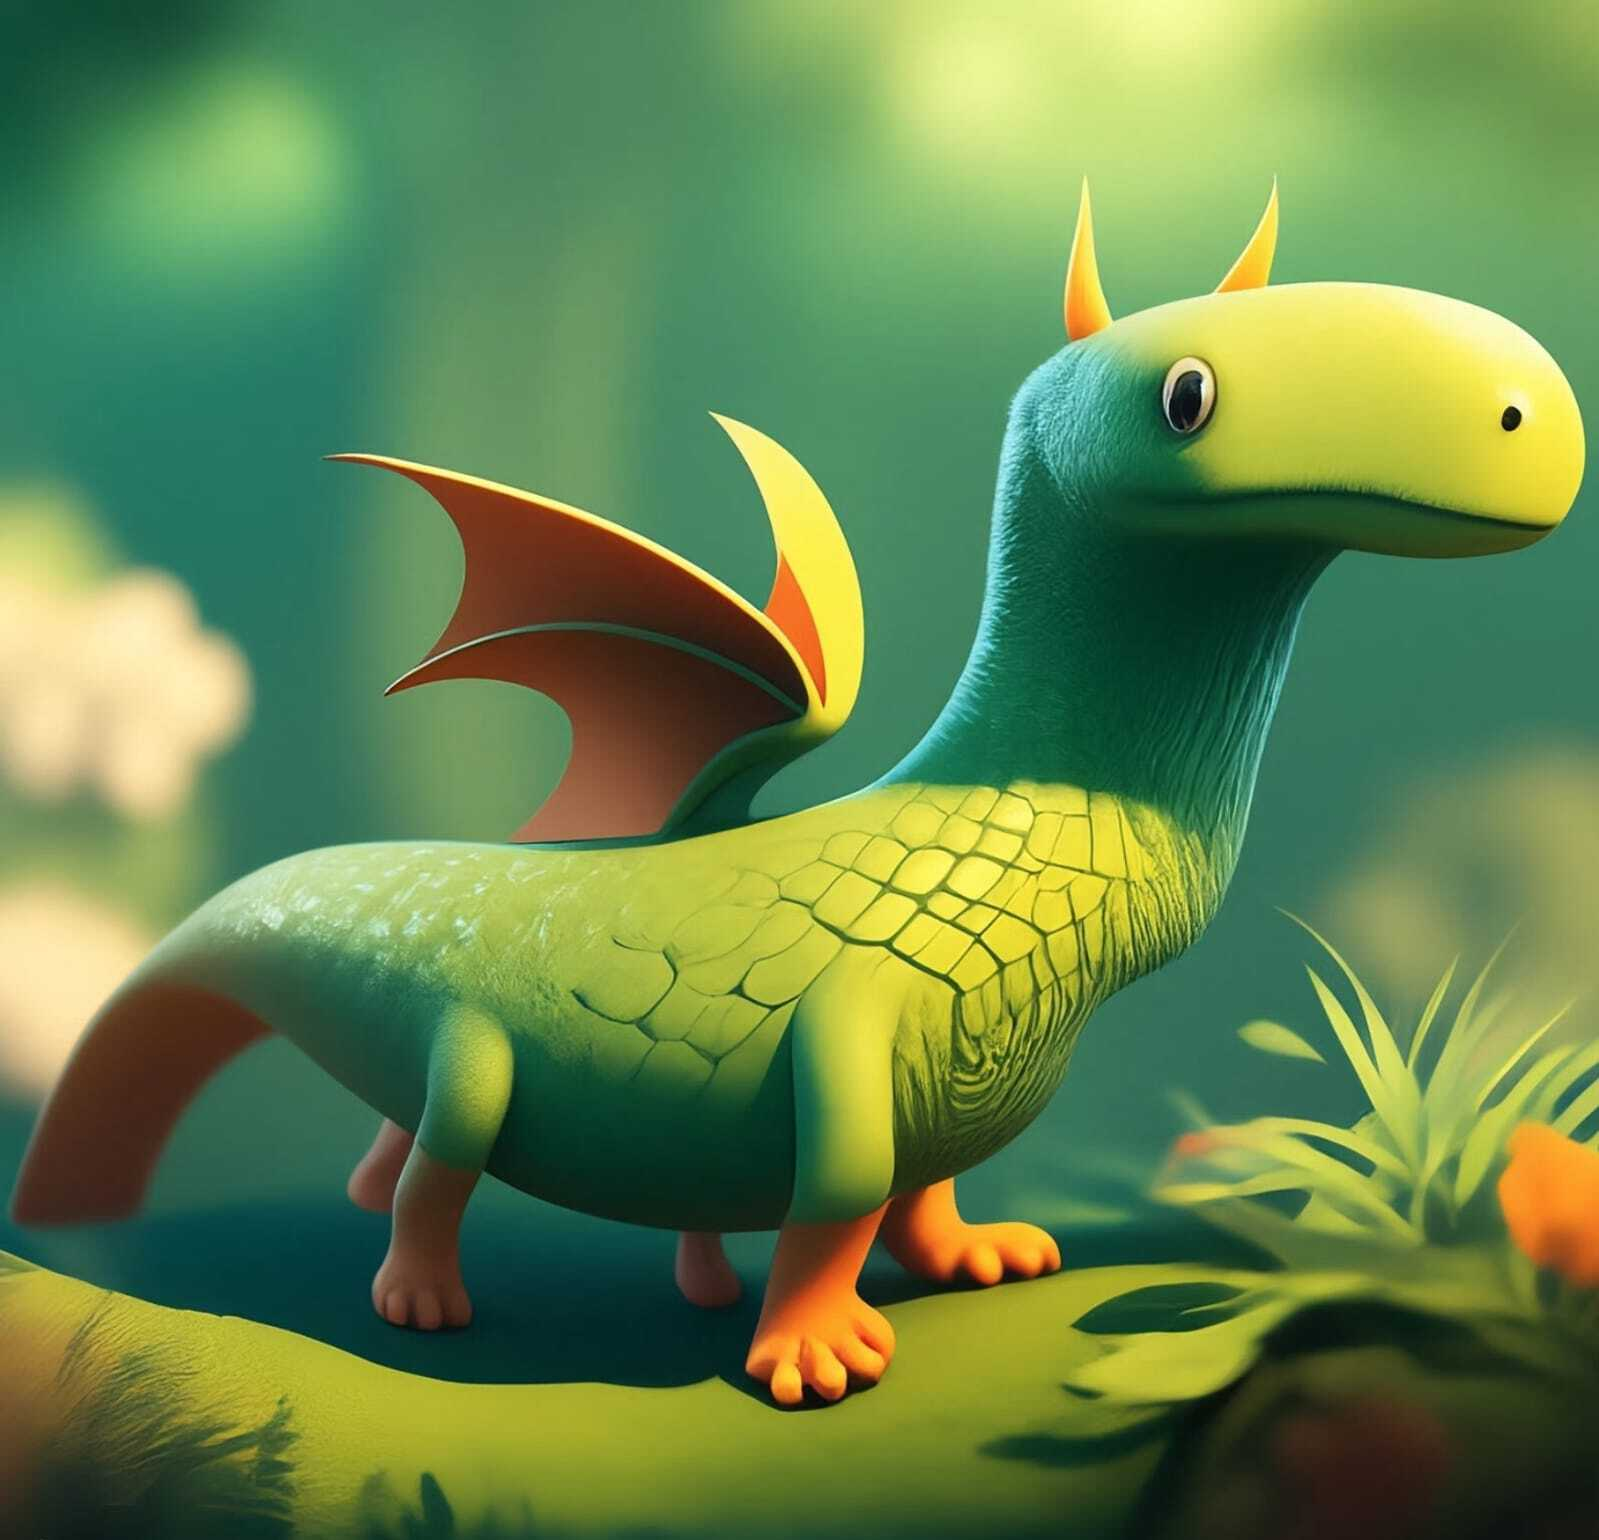
\includegraphics[width=6cm]{cover}
\end{center}
}

% theorem commands
\newtheoremstyle{c_remark}
	{}	% Space above
	{}	% Space below
	{}% Body font
	{}	% Indent amount
	{\bfseries}	% Theorem head font
	{}	% Punctuation after theorem head
	{.5em}	% Space after theorem head
	{\thmname{#1}\thmnumber{ #2}\thmnote{ \normalfont{\text{(#3)}}}}	% head content
\newtheoremstyle{c_definition}
	{3pt}	% Space above
	{3pt}	% Space below
	{}% Body font
	{}	% Indent amount
	{\bfseries}	% Theorem head font
	{}	% Punctuation after theorem head
	{.5em}	% Space after theorem head
	{\thmname{#1}\thmnumber{ #2}\thmnote{ \normalfont{\text{(#3)}}}}	% head content
\newtheoremstyle{c_plain}
	{3pt}	% Space above
	{3pt}	% Space below
	{\itshape}% Body font
	{}	% Indent amount
	{\bfseries}	% Theorem head font
	{}	% Punctuation after theorem head
	{.5em}	% Space after theorem head
	{\thmname{#1}\thmnumber{ #2}\thmnote{ \text{(#3)}}}	% head content

\ifcsname c@english\endcsname
	\theoremstyle{plain}
	\newtheorem{theorem}{Theorem}[section]
	\newtheorem{lemma}[theorem]{Lemma}
	\newtheorem{proposition}[theorem]{Proposition}
	\newtheorem*{proposition*}{Proposition}
	%\newtheorem{corollary}[theorem]{אין חלופה עברית}

	\theoremstyle{definition}
	\newtheorem{definition}[theorem]{Definition}
	\newtheorem*{definition*}{Definition}
	\newtheorem{example}{Example}[section]
	\newtheorem{exercise}{Exercise}[section]

	\theoremstyle{remark}
	\newtheorem*{remark}{Remark}
	\newtheorem*{solution}{Solution}
	\newtheorem{conclusion}[theorem]{Conclusion}
	\newtheorem{notation}[theorem]{Notation}
\else
	\theoremstyle{c_plain}
	\newtheorem{theorem}{משפט}[section]
	\newtheorem{lemma}[theorem]{למה}
	\newtheorem{proposition}[theorem]{טענה}
	\newtheorem*{proposition*}{טענה}
	%\newtheorem{corollary}[theorem]{אין חלופה עברית}

	\theoremstyle{c_definition}
	\newtheorem{definition}[theorem]{הגדרה}
	\newtheorem*{definition*}{הגדרה}
	\newtheorem{example}{דוגמה}[section]
	\newtheorem{exercise}{תרגיל}[section]

	\theoremstyle{c_remark}
	\newtheorem*{remark}{הערה}
	\newtheorem*{solution}{פתרון}
	\newtheorem{conclusion}[theorem]{מסקנה}
	\newtheorem{notation}[theorem]{סימון}
\fi

% Questions related commands
\newcounter{question}
\setcounter{question}{1}
\newcounter{sub_question}
\setcounter{sub_question}{1}

\ifcsname c@english\endcsname
	\newcommand{\question}[1][0]{
		\ifthenelse{#1 = 0}{}{\setcounter{question}{#1}}
		\section{Question \arabic{question}}
		\addtocounter{question}{1}
		\setcounter{sub_question}{1}
	}

	\newcommand{\subquestion}[1][0]{
		\ifthenelse{#1 = 0}{}{\setcounter{sub_question}{#1}}
		\subsection{Part \alph{sub_question}}
		\addtocounter{sub_question}{1}
	}
\else
	\newcommand{\question}[1][0]{
		\ifthenelse{#1 = 0}{}{\setcounter{question}{#1}}
		\section{שאלה \arabic{question}}
		\addtocounter{question}{1}
		\setcounter{sub_question}{1}
	}

	\newcommand{\subquestion}[1][0]{
		\ifthenelse{#1 = 0}{}{\setcounter{sub_question}{#1}}
		\subsection{סעיף \localecounter{letters.gershayim}{sub_question}}
		\addtocounter{sub_question}{1}
	}
\fi

% import lua and start of document
\directlua{common = require ('../common')}

\GetEnv{AUTHOR}

% headers
\author{\AUTHOR}
\date\today

\title{Exercise 3 Answer Sheet --- Logic Theory (2), 80424}

\begin{document}
\maketitle
\maketitleprint{}

\question{}
Let $T = \operatorname{Th}(\hat{\NN})$
We will show that $T$ has $2^\omega$ non-isomorphic countable models.
\begin{proof}
	Let us define $P \subseteq \hat{\NN}$ the set of prime numbers.
	We assume that $S \subseteq P$ is some set.
	We enrich the language by a new constant symbol, $c$.
	Let $T_S = T \cup \{ \exists x, (x \cdot p = c) \land \lnot (\exists y, y \cdot p = x) \mid p \in S \}$, namely extension of $T$ such that $c = \prod_{p \in S} p$.
	$T_S$ is finitely satisfiable by $\hat{\NN}$ as for every finite $S$, $\prod_{p \in S} p \in \NN$, then by compactness $T_S$ is also satisfiable.
	It follows that there is a model $\Mm_S \models T_S$ over $L \cup \{ c \}$, then it is also a model of $T$ by reduction of the language.
	
	Let $S \ne S'$ be subsets of $P$ and let $\Mm, \Nn$ be some of their respective models.
	We will show that $\Mm \not\simeq \Nn$.
	It is clear for $L \cup \{ c \}$-isomorphisms, as there is $p \in S \setminus S'$ (without loss of generality) such that $\Mm \models p \mid c$ but $\Nn \not\models p \mid c$.
	By the last claim we can deduce that if there was such $L$-isomorphism, then for $c^\Mm$ there would be a contradiction, meaning there is no such isomorphism.

	We know that $P \subseteq \NN$, and that this set is not finite, then $|P| = \omega$, it derives that there are $|2^P| = 2^\omega$ non-isomorphic models $\Mm_S \models T$.
\end{proof}

\question{}
Let $F$ be an infinite field, and let $L_{F \operatorname{VS}}$ be the language of vector spaces over $F$.
Let $V \subseteq U$ be two non-trivial vector spaces over $F$, we will show that $V \prec U$.
\begin{proof}
	Let $P$ be a $L_{F \operatorname{VS}}$-disjoint unary relation symbol to $L_{F \operatorname{VS}}$, and let us define $L' = L_{F \operatorname{VS}} \cup \{ P \}$.
	We extend $U$ to $L'$ by $P^U(x) \iff x \in V$, namely $U'$.
	For every $\psi(x_0, \ldots, x_{n - 1}) \in \operatorname{form}_{L \operatorname{VS}}$, let $\varphi_{\psi}(x_0, \ldots, x_{n - 1}) = \psi(x_0, \ldots, x_{n - 1}) \land P(x_0) \land \ldots \land P(x_{n - 1})$,
	a formula such that $U' \models \psi \iff V \models \psi$.
	It follows that there is a theory $T$ such that $U' \models T \iff V \prec U$, meaning that $T$ testifies to elementary substructure of $V$ in $U$.

	Assuming that $|F| = \kappa$ we use upward Löwenheim–Skolem theorem to extend $U'$ to a model $U''$ such that $|U''| > \kappa$ and $U' \prec U''$.
	We define $V'' = P^{U''}$, meaning that $V''$ is the extension of $V$.
	We note that $|F| < |U''|, |V''|$, hence both spaces are infinite dimensional.
	From question 1 of exercise 2 we infer that indeed $V'' \prec U''$, implying that $U'' \models T$, then $U' \models T$ as well, which lead us to the conclusion that $V \prec U$, as intended.
\end{proof}

\question{}
Let $\Mm$ be the model $\langle \QQ(\pi); + \rangle$,
we will show that the function $f_\pi : \QQ(\pi) \to \QQ(\pi)$ such that $f_\pi(u) = \pi u$ is not definable in $\Mm$.
\begin{proof}
	We will show that there is no formula $\varphi(x, y) \in \operatorname{form}_L$ such that $f_\pi$ is definable as the separation of $\varphi$ on $M$, meaning that $\varphi(x, y) \iff y = \pi \cdot x$.
	We assume toward a contradiction that such a formula indeed exists.
	Let $\Nn \succ \Mm$ be an elementary extension such that $|M| < |N|$, namely a model of larger cardinality, which derived from Löwenheim–Skolem theorem.
	We fix some $e \in N \setminus M$, there is indeed one as $|N \setminus M| = |N|$.
	Let $B = M \cup \{ e \}$ and $\Nn' = \Sp B$, the vector space over the field $\QQ$.
	It directly follows that $M \subseteq N'$, as well the language enrichment $\Mm'$ of $\Mm$ to vector spaces over $\QQ$ fulfills $\Mm' \prec \Nn'$ by the last question.
	We reduce the language to infer that $\Mm \prec \Nn'$ as well.
	We assumed that $\Mm \models \forall x \exists y, \varphi(x, y)$ (the function condition over the formula $\varphi$), it follows that $\Nn' \models \forall x \exists y, \varphi(x, y)$ as well.
	In particular, $\Nn' \models \exists y, \varphi(e, y)$, meaning that $y = \pi \cdot e$, but $e \notin M$ and is not closed to multiplication by $\pi$, which implies that $\pi \cdot e \notin \Nn'$,
	a contradiction to the assumption that $\varphi$ exists.
\end{proof}

\question{}
\subquestion{}
We will show that PA proves that the addition is associative and commutative.
\begin{proof}
	we will prove that
	\[
		\operatorname{PA} \models \forall x, y (S(x + y) = S(x) + y)
		\tag{C1}
	\]
	by induction over $y$.
	For $y = 0$ it derives that $S(x + 0) = S(x) = S(x) + 0$ from axiom N3.
	If $\operatorname{PA} \models \forall x, (S(x + n) = S(x) + n)$ then,
	\begin{align*}
		\forall x, (S(x + n) = S(x) + n)
		& \iff \forall x, (S(S(x + n)) = S(x) + S(n)) \\
		& \iff \forall x, (S(x + S(n)) = S(x) + S(n))
	\end{align*}
	Directly by axiom N4.

	Let $\varphi(y) = \forall x, z (x + (y + z) = (x + y) + z)$, and $\psi = \forall y \psi(y)$ be the sentence that testifies to associativity, we will show that $\operatorname{PA} \models \psi$,
	by showing that $\operatorname{Ind}(\varphi)$ holds.
	$\operatorname{PA} \models \varphi(0)$ directly by the axioms N3 and N4.
	Let us assume that $\varphi(n)$ holds, we will show that $\varphi(S(n))$ holds as well,
	\begin{align*}
		\operatorname{PA} \models \varphi(n)
		& \iff \forall x, z (x + (n + z) = (x + n) + z) \\
		& \overset{\text{N1}}{\iff} \forall x, z (S(x + (n + z)) = S((x + n) + z)) \\
		& \overset{\text{N4, C1}}{\iff} \forall x, z (x + S(n + z) = S(x + n) + z) \\
		& \iff \forall x, z (x + (S(n) + z) = (x + S(n)) + z) \\
		& \iff \varphi(S(n))
	\end{align*}
	We conclude by induction axiom scheme that indeed $\operatorname{PA} \models \psi$.

	Let $\varphi(x) = \forall y (x + y = y + x)$ and $\psi = \forall x, \varphi(x)$, sentence such that $\operatorname{PA} \models \psi$ if and only if PA is commutative.
	We will show that $\operatorname{PA} \models \operatorname{Ind}(\varphi)$.
	For $x = 0$, $0 + y = S(0 + y') = \cdots = S(S(\cdots S(0 + 0))) = y = y + 0$ by axioms N3 and N4.
	Let us assume that $\varphi(n)$ holds, then,
	\begin{align*}
		\operatorname{PA} \models \varphi(n)
		& \iff \forall y (n + y = y + n) \\
		& \overset{\text{N1}}{\iff}  \forall y (S(n + y) = S(y + n)) \\
		& \overset{\text{N4, C1}}{\iff}  \forall y ((S(n) + y) = y + S(n)) \\
		& \iff \operatorname{PA} \models \varphi(S(n))
	\end{align*}
	It follows that $\operatorname{Ind}(\varphi)$ holds, meaning that $\operatorname{PA} \models \psi$.
\end{proof}

\subquestion{}
We will show that PA proves that $(+, \cdot, \le)$ is a semi-ring, namely $+, \cdot$ are associative and commutative, $0, 1$ are neutral and $\le$ is linear order.
\begin{proof}
	associativity and commutativity of $+$ was shown in the first part, the proof for $\cdot$ is similar.
	By N3 and N5 we infer that $0, 1$ are indeed neutral elements.
	
	We move to show $\le$ is a linear order.
	From N9, $\le$ is reflexive.
	To show transitivity we use induction, for the base N7 and for the step iterative usage of N8.
	For linearity we use N9.
	We also need to show that both $+$ and $\cdot$ are order-preserving for $\le$.
	This statement is proven in induction over the added value to both sides of every inequality.
\end{proof}

\end{document}
